Here, we will define some concepts related to the term "game". The following discussion is not comprehensive, it is only intended to clarify and narrow down our definition of gamification. 

\begin{itemize}
\item Playful design or gameful design
\end{itemize}
Playful design is using game-based aesthetics or limited usability
based on game elements in non-game contexts with the purpose of
drawing the user's attention [1]. These elements are used to amuse
users and cause an emotional response. One successful example is
Twitter’s page knows as “Fail Whale” (Figure 1-a). Whenever
there is an overload on the servers, instead of a boring page with
some standard error message, users are presented with a drawing of
a dozen birds, twitters, trying to lift a whale.

\begin{itemize}
\item Serious games
\end{itemize}
Serious games are games designed for non-recreational
environments and for educational purposes [16]. The term
“serious” is employed because these games can focus on areas as
diverse as economics, education, health, industry, military,
engineering, and politics. In environments created by applying
serious game concepts, it is possible to simulate real-world
situations without incurring in eventual costs and risks. The main
goal of this sort of training-environment is to convey information
to the user [31]. The Virtual Incident Management Training System
(Figure 1-c) is a multiplayer training environment designed for
training professionals that need to act swiftly in case of accident on
highways, such as paramedics and policemen [37].

\begin{itemize}
\item Video games or digital games
\end{itemize}
Video Games or Digital Games are systems in which users are
engaged in resolving abstract conflicts and challenges, under
predetermined rules [36]. In this scenario the game continuously
offers interactivity and feedback to the user, which often result in
an emotional reaction. Figure 1-d shows a screenshot of the game
New Super Mario Bros.Wii© whose main character, Mario, is
considered one of the most iconic video game characters.

\begin{itemize}
\item Gamification
\end{itemize}
As mentioned, it consists of using game developing techniques in
non-game environments, such as social networks [16]. The
techniques and resources used in digital games have elements
capable of motivating the user, hold his interest and challenge him
to solve problems. In gamification approaches, these elements are
not the center of the system, but have the purpose of motivating
users to use it [28]. Foursquare application (Figure 1-b) is an
example of a gamified system. Foursquare is a location-based
social network, which reached one billion “check-ins” in 2011.
Foursquare allows users to check-in at venues using a device specific
front-end to the application (e.g., mobile website), each
check-in might award the user with user-points or “badges”.
It is worth to point out that the current work focus on covering
research that explicitly match our definition of Gamification.
Therefore, we are not considering research based on serious games,
video games, playful design and other uses of game concepts in
educational contexts.\todo{refazer a figura com coisas atuais}

\begin{figure}[h!]
\caption{Examples of (a) playful design, (b) gamification, (c)
serious games and (d) digital games.}
\centering
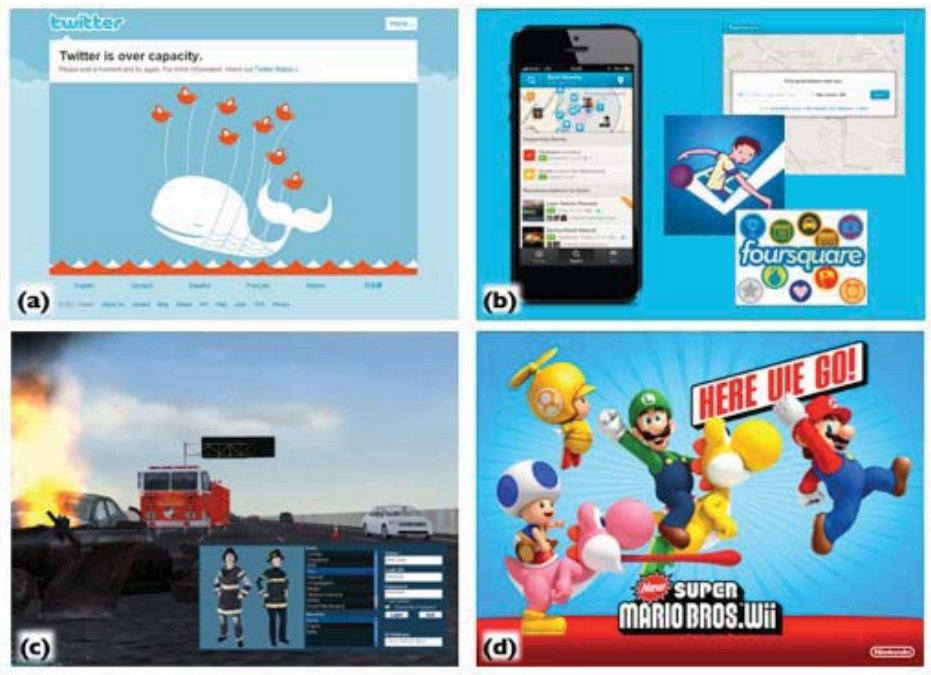
\includegraphics[width=\textwidth]{gameful_design}
\end{figure}